%
% To start the document, use
%  \levela{...}
% For lover level, sections use
%  \levelb{...}
%  \levelc{...}
%
\levela{The ARTS concept}
 \label{sec:concept}

%
% Document history, format:
%  \starthistory
%    date1 & text .... \\
%    date2 & text .... \\
%    ....
%  \stophistory
%
\starthistory
  000616 & Created by Stefan Buehler, based on my DPG2000 poster.\\
  011121 & Practical hints added by Stefan Buehler.
\stophistory

%
% Symbol table, format:
%  \startsymbols
%    ... & \verb|...| & text ... \\
%    ... & \verb|...| & text ... \\
%    ....
%  \stopsymbols
%
%

%
% Introduction
%
This section describes the basic ideas underlying ARTS. It also
introduces some terminology. You should read it if you want
to understand how the program works and how it can be used
efficiently. At the end of the chapter, there is also some practical
information about useful command line parameters and such things. 


\levelb{Introduction}
%====================
\label{sec:concept:intro}

The number of satellite sensors in the millimeter and sub-millimeter
spectral range is rapidly growing. They use various frequency
bands and observation geometries. Two important groups of
sensors are for example the nadir viewing millimeter wave
sensors like AMSU\footnote{The \textbf{A}dvanced
  \textbf{M}icrowave \textbf{S}ounding \textbf{U}nit is a
  sensor on board the polar orbiting satellites of the
  US-American National Aeronautics and Space Administration.}
and the limb viewing sub-millimeter wave sensors like the
planned SMILES\footnote{The \textbf{S}uperconducting
  Sub-\textbf{Mi}llimeter Wave \textbf{L}imb \textbf{E}mission
  \textbf{S}ounder is a Japanese Sensor which will be flown
  for the first time on the International Space Station.}.

For the data analysis all such sensors require accurate and
fast forward models, which can simulate measurements for a
given atmospheric (and maybe ground) state. Depending on the
objective of the sensor, the measurement will depend for
example on the distribution of atmospheric temperature, water
vapor, ozone, and many other trace gases.

So far, a lot of effort has been wasted in developing
dedicated forward models for different sensors, although all
these models have many features in common. Moreover, existing
models were not easily modifiable and extendable. Hence, it
was decided to develop a new model which emphasizes
modularity, extendibility, and generality.


\levelb{The scope of ARTS}
%====================
\label{sec:concept:scope}

The present version of ARTS is limited to cases where scattering can
be neglected and local thermodynamic equilibrium applies. ARTS has
been developed having passive emission measurements in mind, put pure
transmission (that is, the emission is neglected) observations are
also handled. The forward model can be used to simulate measurements
for all (normal?)  observation geometries: ground-based, nadir
looking, limb sounding and balloon/aircraft measurements. It can be
noted that ARTS handles measurements from a point inside the
atmosphere, such as an aircraft or a balloon, in a downward direction.
ARTS covers so far only monochromatic pencil beam calculations, that
is, no sensor characteristics can be included. This part is presently
covered by the AMI (ARTS Matlab interface) set of Matlab functions 
(see below). Sensor characteristics will be included in ARTS.

Beside providing set of spectra, ARTS calculates weighting functions
for a number of variables. Analytical expressions for the weighting
functions are used for species, continuum absorption and ground
emission, and for temperature if hydrostatic equilibrium is \emph{not}
assumed. Weighting functions are also provided for pointing off-sets,
calibration and temperature (with hydrostatic equilibrium).

For Matlab users there are two accompanying packages called AMI and
Qpack\footnote{AMI is distrubuted by ARTS, while Qpack is a separate
  package} which extends the usage of ARTS considerably. First of all,
AMI has functions to include sensor characteristics in the
calculations. AMI has further functions to read and write ARTS data
file, and various functions that are of general usage. Qpack is an
Matlab environment to perform OEM inversions and producing set of
spectra to test the inversions, where ARTS is used as calculating
engine.



\levelb{Enter: ARTS}
%===================
\label{sec:concept:arts}

The most important notion in ARTS is the \emph{workspace}. All
physical quantities (for example absorption coefficients) are
\emph{workspace variables}. But workspace variables can also be of
a more technical nature, for example various grids. 

The program performs a calculation by executing a list of
\emph{workspace methods}, which are specified in a
controlfile. These workspace methods take workspace variables as
input, and generate workspace variables as output. Additional
input parameters can be specified as \emph{keyword parameters} in
the controlfile (Figure \ref{fig:method}).

\begin{figure}
  \begin{center}
    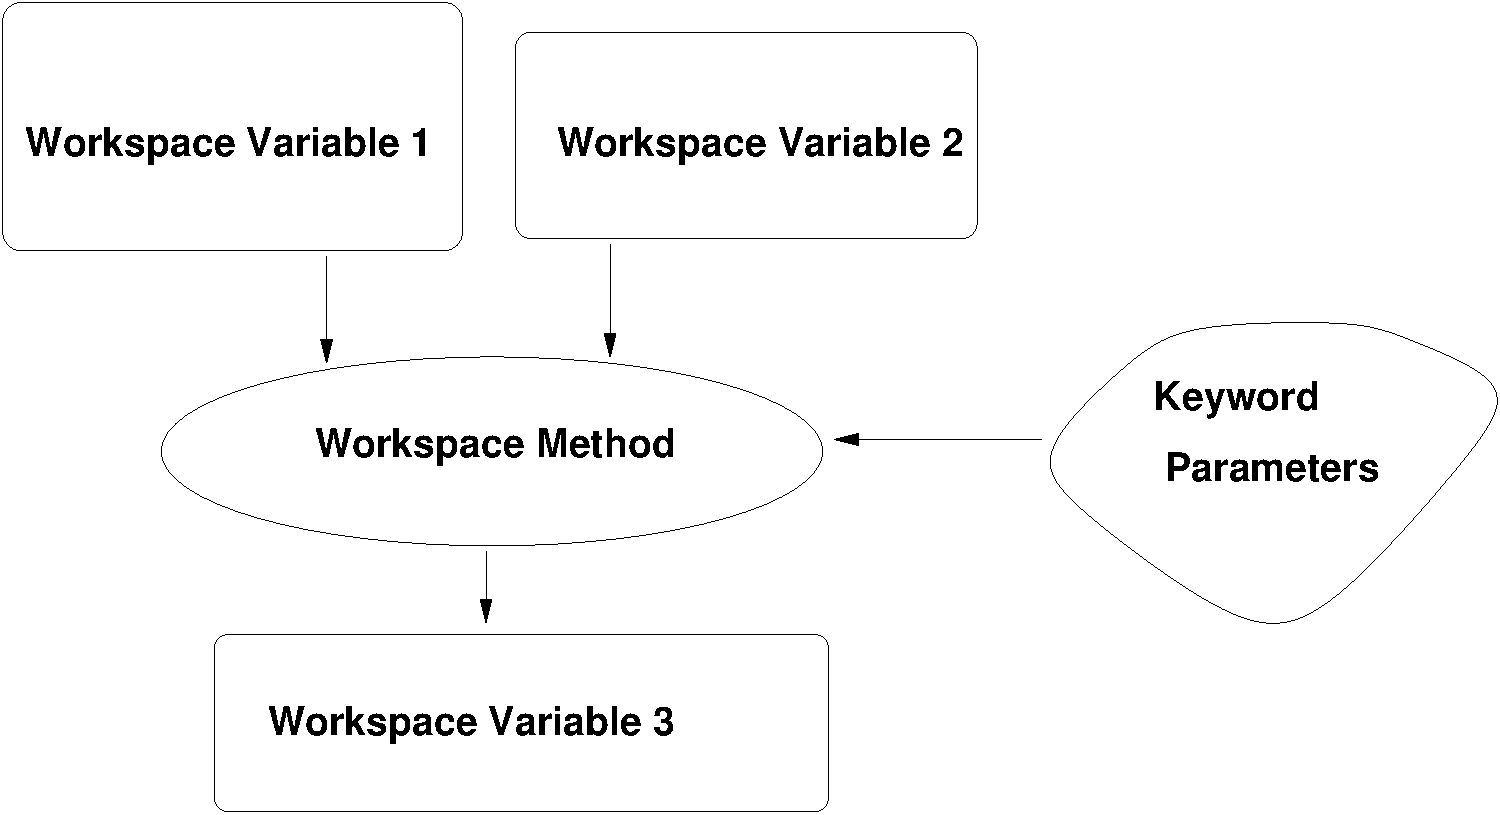
\includegraphics[width=\hsize,draft=false]{method}
    \caption{\emph{Specific}
        workspace methods act on specific workspace variables to
        generate other specific workspace variables. Additional input
        parameters can be specified as keyword parameters in the
        controlfile.}
    \label{fig:method}
  \end{center}
\end{figure}

It is important to note that the controlfile has a fixed and
well-defined syntax. This syntax is understood by the ARTS parser.
The great advantage of this concept is that it is very easy to add
new workspace variables and new workspace methods. The program has
an internal lookup table which lists all workspace methods, as well
as their input variables, output variables, and keyword
parameters. To add a new method, one just has to add an entry to
this lookup table, and write the code for the method itself. No
further changes to the program are necessary. In particular, no
changes to the program logic or to the parser. How such an extension
can be made practically is described in Section \ref{sec:development}.


\levelb{Generic Workspace Methods}
%=================================
\label{sec:concept:generic}

Generic methods (Figure \ref{fig:generic_method}) allow the user of the
program even more freedom than specific methods. A generic method is
for example \verb|VectorReadAscii|, which can be used to read any
workspace variable which is a vector from an ASCII file. For example
\begin{quote}
  \verb|VectorReadAscii(f_mono){"freqeuency_grid.aa"}|
\end{quote}
will read the specified file and generate the workspace variable
\verb|f_grid|.

\begin{figure}
  \begin{center}
    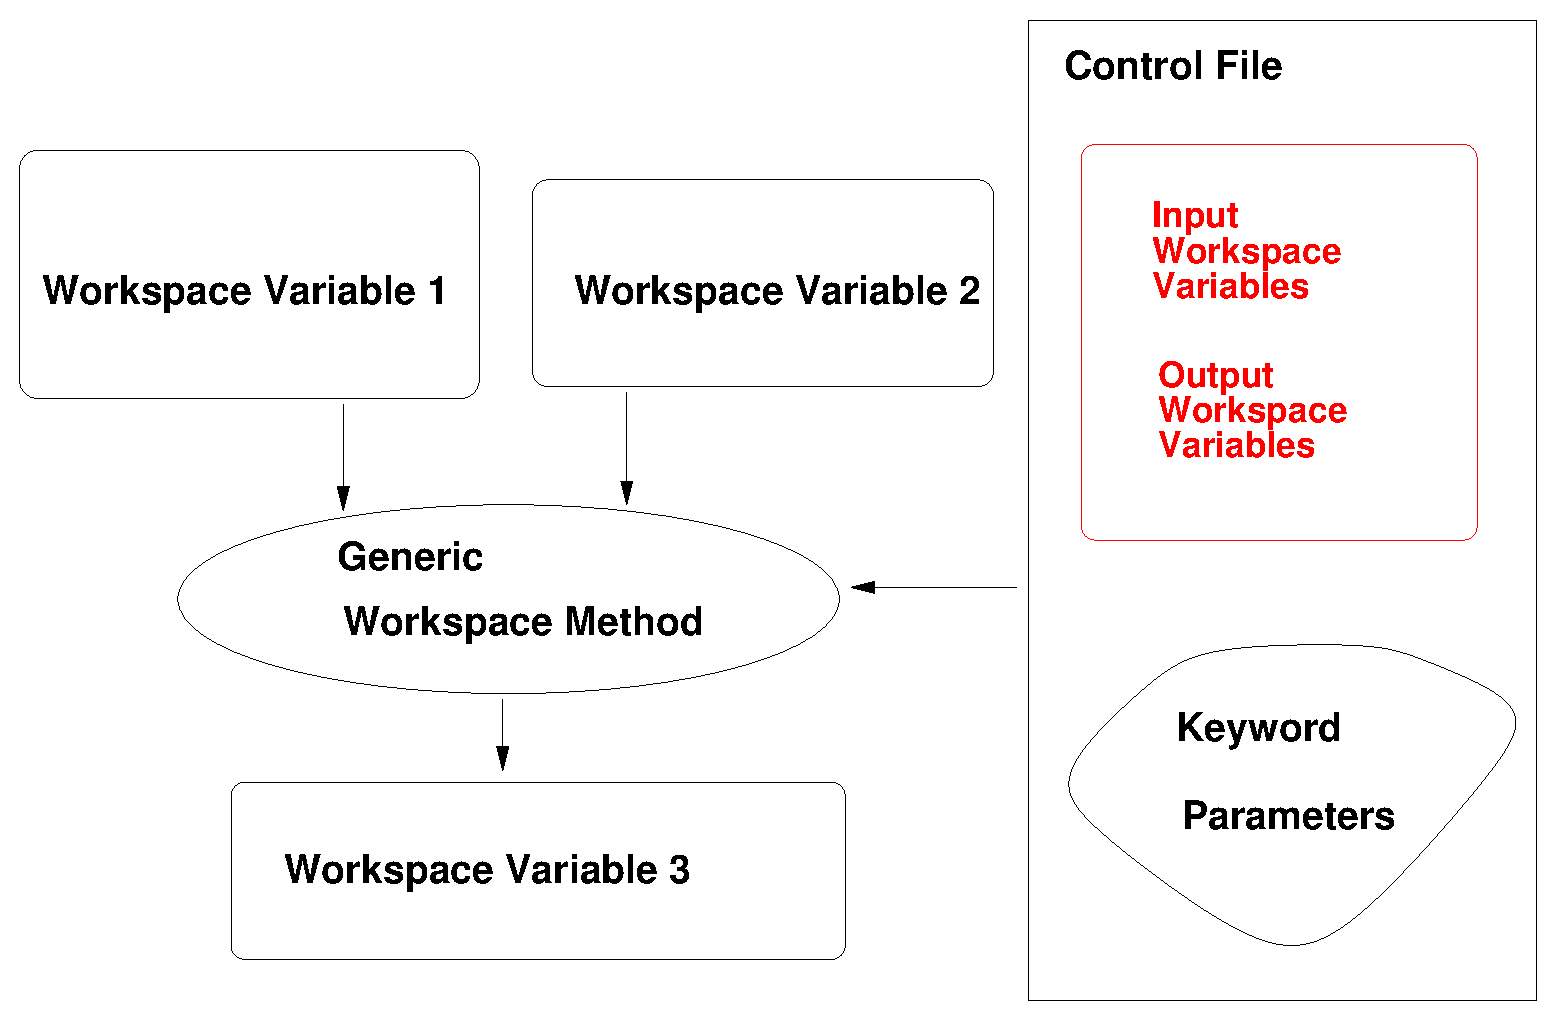
\includegraphics[width=\hsize,draft=false]{generic_method}
    \caption{For \emph{generic}
      workspace methods the workspace variables to act on are
        specified in the controlfile.}
    \label{fig:generic_method}
  \end{center}
\end{figure}

Generic methods are particularly useful for IO operations like in the
example above. No new IO functions are necessary for new workspace
variables, as long as they are of standard types already known to the
program (for example vectors or matrices). 

\levelb{Practical hints}
%=================================
\label{sec:concept:practical}

The subdirectory \verb|examples| of the \verb|doc| directory contains
some example controlfiles. You should study them to learn more about
how the program works. You can also run these controlfiles like this:
\begin{quote}
\begin{verbatim}
  arts absorption_example.arts
\end{verbatim}
\end{quote}
This assumes that you are inside the directory where the controlfiles
are, and that the \verb|arts| executable is in your path.  You can
also run all of the examples, by saying
\begin{quote}
\begin{verbatim}
  make check
\end{verbatim}
\end{quote}

ARTS offers a number of useful command line parameters. In general,
there is a short form and a long form for each parameter. The short
form consists of a minus sign and a single letter, whereas the long
form consists of two minus signs and a descriptive name. To get a full
list, type
\begin{quote}
\begin{verbatim}
  arts -h
\end{verbatim}
\end{quote}
or
\begin{quote}
\begin{verbatim}
  arts --help
\end{verbatim}
\end{quote}
Most useful at the beginning should be the \verb|-d|
(\verb|--describe|), \verb|-m| (\verb|--methods|), \verb|-w|
(\verb|--workspacevariables|), and \verb|-i| (\verb|--input|) flags.
For instance, the \verb|-d| (\verb|--describe|) flag gives you online
documentation for any workspace method or workspace variable. Usage:
\begin{quote}
\begin{verbatim}
  arts -d f_mono
\end{verbatim}
\end{quote}
will print documentation about the workspace variable \verb|f_mono|, which
happens to be the monochromatic frequency grid.

But what methods and variables are available? You can find out by
typing
\begin{quote}
\begin{verbatim}
  arts -m all
\end{verbatim}
\end{quote}
which will list all workspace methods, or by typing 
\begin{quote}
\begin{verbatim}
  arts -w all
\end{verbatim}
\end{quote}
which will list all workspace variables. As you can see, these lists
are quite long. But you can get more specific information:
\begin{quote}
\begin{verbatim}
  arts -m f_mono
\end{verbatim}
\end{quote}
will give you a list of all methods that can generate the workspace
variable \verb|f_mono|. Specific and generic methods are listed
separately. Generic methods are in this case all methods producing a
Vector, since \verb|f_mono| belongs to this group. A similar task is
performed by the \verb|-i| (\verb|--input|) flag, with the difference
that \verb|arts -i f_mono| will list those methods that require
\verb|f_mono| as \emph{input}, whereas \verb|arts -m f_mono| lists
those that produce \verb|f_mono| as output. Finally,
\begin{quote}
\begin{verbatim}
  arts -w absCalc
\end{verbatim}
\end{quote}
will give you all variables required by the method \verb|absCalc|
(the variable \verb|f_mono| happens to be one of them).

Using these command line parameters, it is easy to build up a
controlfile. The trick is, to start at the end. Say you want to
compute absorption coefficients. First of all, you have to find out
in which workspace variable these are stored. Look at the list
produced by \verb|arts -w all|. You can use \verb|arts -d| to look at
some candidates a bit more closely. This way, you will find out that
\verb|abs| is the variable you are looking for.

In the next step, you can use \verb|arts -m abs| to find all methods
that can calculate \verb|abs|. So, you will find the method
\verb|absCalc|. Now you can use \verb|arts -w absCalc| to find out the
required input variables of that method. Then you can use the
\verb|-m| flag again, to find the methods producing these variables,
and so on.

%%% Local Variables: 
%%% mode: latex
%%% TeX-master: "uguide"
%%% End: 
